\section[rel]{Relation Neural Networks / Network Architectures}

\begin{frame}
\frametitle{Architectures with builtin properties}
\begin{itemize}
\item Convolutional neural network: Spatial Invariance
\item Recurrent neural network: Sequential Dependency
\item Relation neural network: Relations between objects
\end{itemize}
\textbf{$\Rightarrow$ dedicated architectures reduce complexity through weight-sharing}

\vspace{-1em}
\begin{align*}
\mathrm{RN}(o_1, o_2, \dots, o_n) &= f_\phi \left( \sum_{i,j} g_\Theta(o_i, o_j) \right)
\end{align*}

Possible relations: Are there two objects ...
\begin{itemize}
\item ... of the same size?
\item ... with the same color?
\item ... with a common vertex?
\end{itemize}

\end{frame}

\begin{frame}
\frametitle{Example: Super-human performance on CLEVR}
\begin{center}
\vspace{-0.5em}
      \begin{tikzpicture}
          \node[anchor=center,inner sep=0]  at (0, 0) {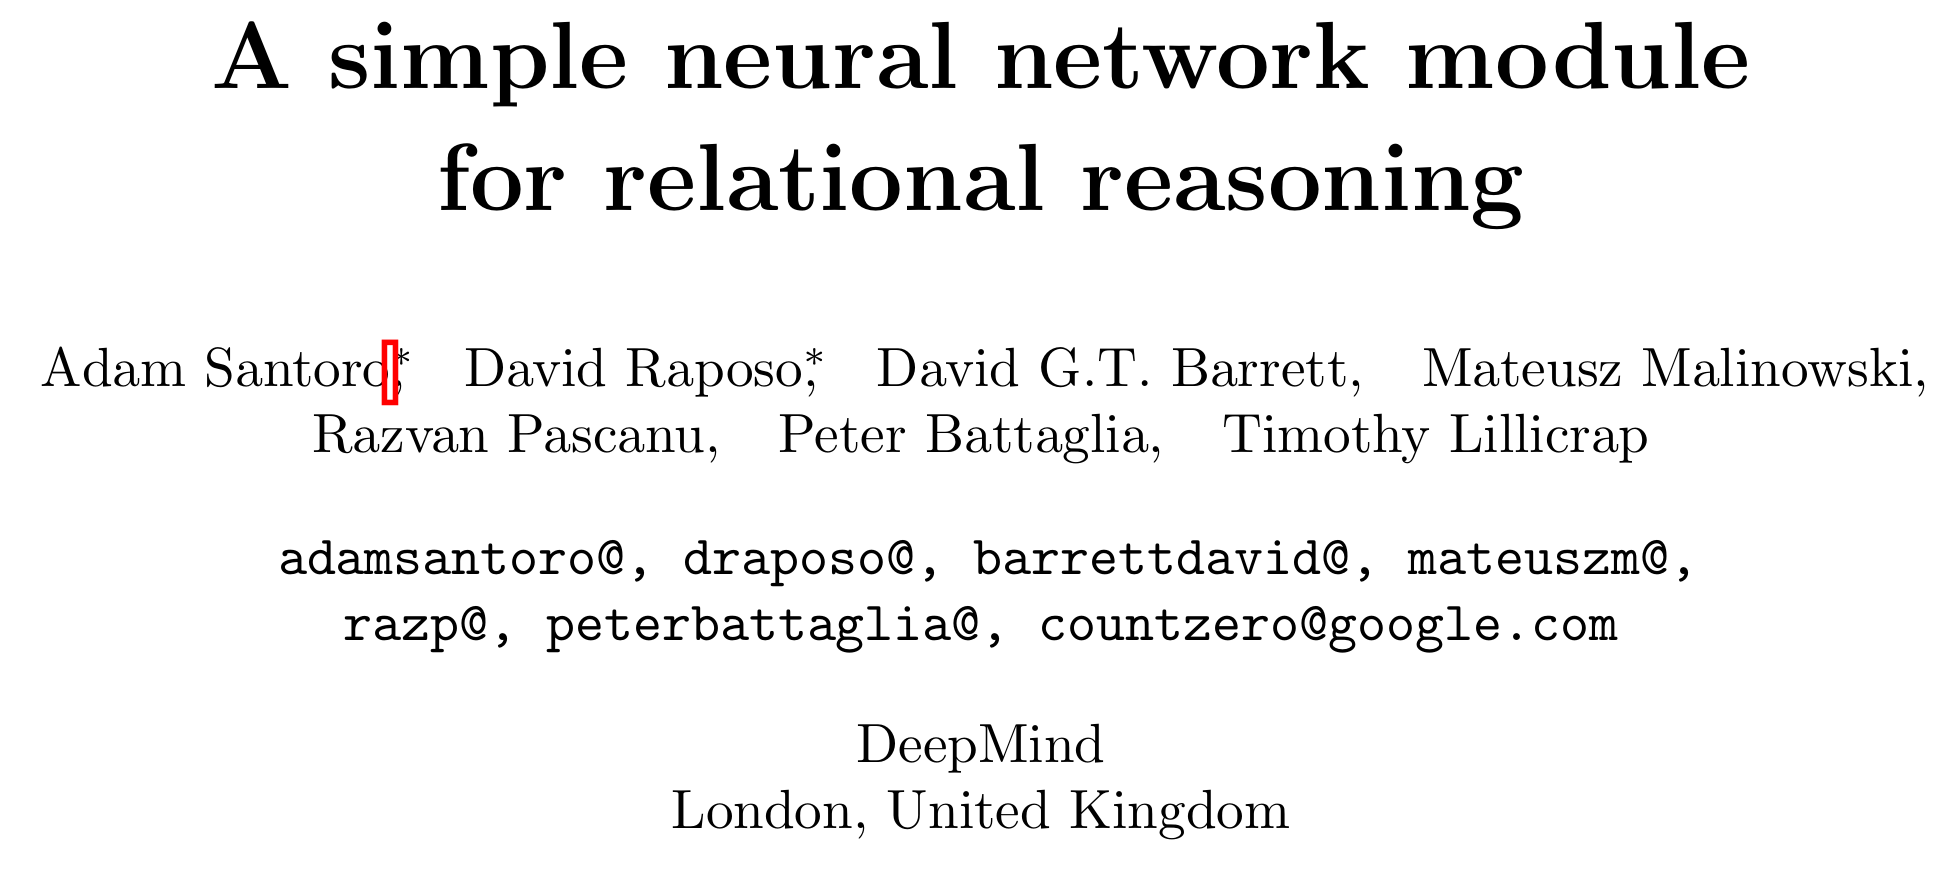
\includegraphics[height=0.3\textheight]{rel_paper.png}};
          \node[anchor=center,inner sep=0]  at (0, -4) {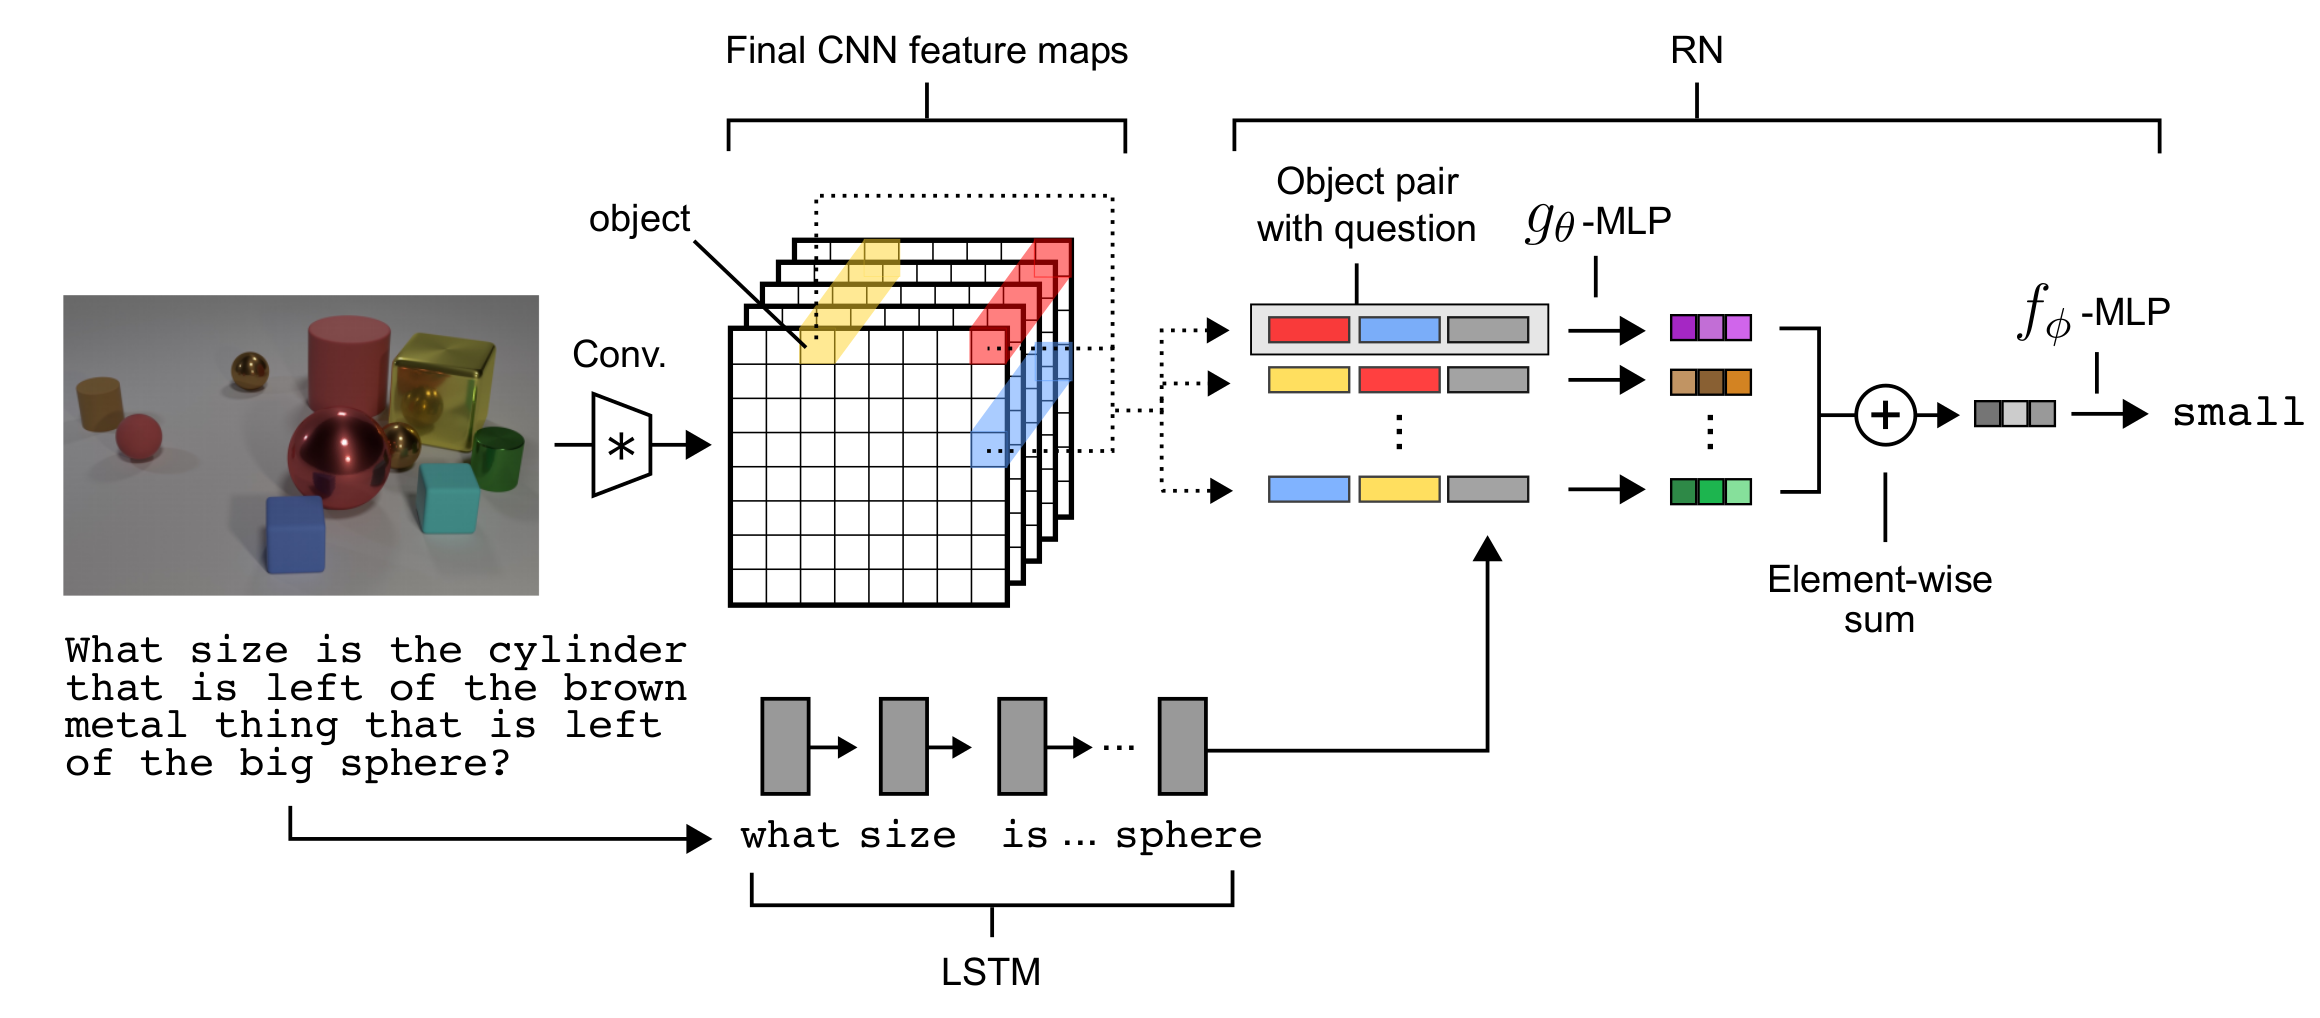
\includegraphics[height=0.5\textheight]{rel_network.png}};
      \end{tikzpicture}
      \end{center}
\end{frame}
